\chapter{Background}
\Rapture is a platform system that can be used to build applications that are scalable,
distributed, consistent and coordinated. At its heart \Rapture is simply a well defined
set of libraries with an external facing api that provides an abstraction to a number
of fundamental concepts. This document describes the APIs of \Rapture in detail from the
perspective of a programmer - alongside each API call are sections on their use within
\Rapture and typical use cases for that API or API set.

The general architecture of a \Rapture system is reproduced in Figure~\vref{fig:RaptureDiagram}.

\begin{figure}[htb]
\centering
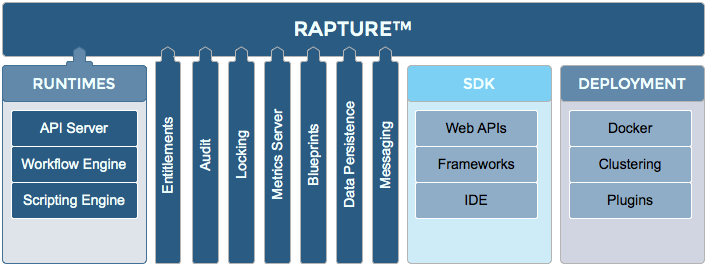
\includegraphics[scale=0.5]{Graphics/rapturecore}
\caption{Rapture Component Parts}
\label{fig:RaptureDiagram}
\end{figure}

Applications that interact with \Rapture, or are \emph{hosted} on \Rapture will
use the \Rapture API to interact with this underlying framework. The goal of
the \Rapture API is that the interaction with \Rapture is invariant to the location
of the application -- the API looks \emph{the same} no matter where the application
resides.

This document presents an overview of \Rapture and its scripting language \Reflex. The first
part contains more general background to \Rapture and presents an overview of its parts. The second
part is a detailed description of the API calls that can be made of a \Rapture system. Finally the third
part presents the \Reflex scripting language.
